% \begin{problem}[1]
%   Evaluate $\displaystyle\iiint_E 3y \,\dd{V}$ where $E$ is the solid bounded by the cylinder $y = \sqrt{x}$ and the planes $y = x$, $z = -3$, and $z = x + y$.
% \end{problem}

% \begin{proof}[Solution]
%   Graphing the bounds on the $xy$-plane gives us
%   \begin{center}
%     \begin{tikzpicture}
%       \begin{axis}[
%         axis lines = center,
%         xlabel = $x$,
%         ylabel = $y$,
%         xmin = -0.5, xmax = 1.5,
%         ymin = -0.5, ymax = 1.5,
%         xtick = {0, 1},
%         ytick = {0, 1},
%         xticklabels = {$0$, $1$},
%         yticklabels = {$0$, $1$},
%         ]
%         \addplot[domain=0:1.5, samples=1000]{sqrt(x)};
%         \addplot[domain=-0.5:1.5]{x};
%       \end{axis}
%     \end{tikzpicture}
%   \end{center}

%   Clearly, from the graph, the bounds for $x$ are $0 \leq x \leq 2$ and for $y$
%   are $x \leq y \leq \sqrt{x}$. The bounds for $z$ are $-3 \leq z \leq x + y$.
%   Expanding the triple integral into an iterated integral gives us
%   \begin{align*}
%     \iiint_E 3y \,\dd{V} &= \int_0^1 \int_x^{\sqrt{x}} \int_{-3}^{x+y} 3y \,\dz \,\dy \,\dx \\
%                          &= \int_0^1 \int_x^{\sqrt{x}} 3yz \bigg\rvert_{-3}^{x+y} \,\dy \,\dx \\
%                          &= \int_0^1 \int_x^{\sqrt{x}} 3y(x + y + 3) \,\dy \,\dx \\
%                          &= \int_0^1 \int_x^{\sqrt{x}} 3y^2 + 3yx + 9y \,\dy \,\dx \\
%                          &= \int_0^1 \left. y^3 + \frac{3y^2x}{2} + \frac{9y^2}{2} \right\rvert_x^{\sqrt{x}} \,\dy \,\dx \\
%                          &= \int_0^1 \left(x^{\sfrac{3}{2}} + \frac{3x^2}{2} + \frac{9x}{2}\right) - \left(x^3 + \frac{3x^3}{2} + \frac{9x^2}{2}\right) \,\dx \\
%                          &= \int_0^1 x^{\sfrac{3}{2}} - \frac{5x^3}{2} - 3x^2 + \frac{9x}{2} \,\dx \\
%                          &= \left. \frac{2}{5}x^{\sfrac{5}{2}} - \frac{5x^4}{8} - x^3 + \frac{9x^2}{4} \right\rvert_0^1 \\
%                          &= \frac{2}{5} - \frac{5}{8} - 1 + \frac{9}{4} = \frac{41}{40}
%   .\qedhere\end{align*}
% \end{proof}

\begin{problem}[2]
  For any continuous $f(x, y, z)$, write $\displaystyle\iiint_E f(x, y, z) \,\dd{V}$ as an iterated integral in the six orders of integration where $E$ is a solid bounded by the surfaces $z = 0$, $x = 0$, $y + 2z = 2$, and $y = \sqrt{x}$.
  Clearly sketch the solid and each of the projections of E onto the coordinate planes.
\end{problem}

\begin{proof}[Solution]
  For the $xy$-plane, we get the following functions $y = 2$, $x = 0$, and $y =
  \sqrt{x} \implies x = y^2$. Finding the intersection point of $y = 2$ and $y =
  \sqrt{x}$ gives us $x = 4$. They intersect at $(4, 2)$. The graph is shown in
  figure \ref{fig:xy_plane}.

  For the $yz$-plane, we get the following functions $z = 1 - \sfrac{y}{2}
  \implies y = 2 - 2z$ and $z = 0$. Solving for their intersections gives us $y
  = 0$ and $z = 0$. They intersect at $(0, 0)$ and $(2, 0)$. The graph is shown
  in figure \ref{fig:yz_plane}.

  For the $xz$-plane, we get the following functions $z = -\sfrac{\sqrt{x}}{2} +
  1$ (since $y = \sqrt{x}$) and $z = 0$. Solving for their intersections gives
  us $x = 4$. They intersect at $(4, 0)$. The graph is shown in figure
  \ref{fig:xz_plane}.

  \begin{figure}[H]
    \begin{subfigure}[b]{0.5\textwidth}
      \centering
      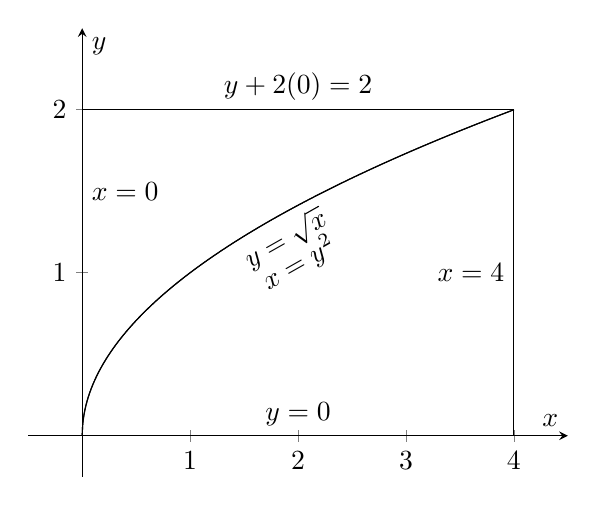
\begin{tikzpicture}
        \begin{axis}[
          axis lines = center,
          xlabel = $x$,
          ylabel = $y$,
          xmin = -0.5, xmax = 4.5,
          ymin = -0.25, ymax = 2.5,
          xtick = {0, 1, 2, 3, 4},
          ytick = {0, 1, 2},
          xticklabels = {$0$, $1$, $2$, $3$, $4$},
          yticklabels = {$0$, $1$, $2$},
          ]
          \node at (axis cs: 0, 1.50) [right] {$x = 0$};
          \node at (axis cs: 2, 0) [above] {$y = 0$};
          \addplot[domain=0:4] {2} node[midway, above] {$y + 2(0) = 2$};
          \addplot[domain=0:4, samples=1000] {sqrt(x)} node[midway, below, sloped] {$y = \sqrt{x}$};
          \addplot[domain=0:4, samples=1000] {sqrt(x)} node[midway, below, sloped, yshift=-1em] {$x = y^2$};
          \draw (4, 0) -- (4, 2) node[midway, left] {$x = 4$};
        \end{axis}
      \end{tikzpicture}

      \caption{$xy$-plane}
      \label{fig:xy_plane}
    \end{subfigure}
    \begin{subfigure}[b]{0.5\textwidth}
      \centering
      \begin{tikzpicture}
        \begin{axis}[
          axis lines = center,
          xlabel = $y$,
          ylabel = $z$,
          xmin = -0.5, xmax = 2.5,
          ymin = -0.25, ymax = 1.25,
          xtick = {0, 1, 2, 3, 4},
          ytick = {0, 1, 2},
          xticklabels = {$0$, $1$, $2$, $3$, $4$},
          yticklabels = {$0$, $1$, $2$},
          ]
          \node at (axis cs: 0, 0.50) [right] {$y = 0$};
          \node at (axis cs: 1, 0) [above] {$z = 0$};
          \addplot[domain=0:2] {1 - x/2} node[midway, above, sloped] {$z = 1 - \sfrac{y}{2}$};
          \addplot[domain=0:2] {1 - x/2} node[midway, above, sloped, yshift=1em] {$y = 2 - 2z$};
        \end{axis}
      \end{tikzpicture}

      \caption{$yz$-plane}
      \label{fig:yz_plane}
    \end{subfigure}

    \begin{subfigure}[b]{\textwidth}
    \end{subfigure}

    \begin{subfigure}[b]{\textwidth}
      \centering
      \begin{tikzpicture}
        \begin{axis}[
          axis lines = center,
          xlabel = $x$,
          ylabel = $z$,
          xmin = -0.5, xmax = 4.5,
          ymin = -0.25, ymax = 1.25,
          xtick = {0, 1, 2, 3, 4},
          ytick = {0, 1, 2},
          xticklabels = {$0$, $1$, $2$, $3$, $4$},
          yticklabels = {$0$, $1$, $2$},
          ]
          \node at (axis cs: 0, 0.50) [right] {$x = 0$};
          \node at (axis cs: 2, 0) [above] {$z = 0$};
          \addplot[domain=0:4, samples=1000] {-sqrt(x)/2 + 1} node[midway, above, sloped] {$z = -\sfrac{\sqrt{x}}{2} + 1$};
          \addplot[domain=0:4, samples=1000] {-sqrt(x)/2 + 1} node[midway, above, sloped, yshift=1em] {$x = (2 - 2z)^2$};
        \end{axis}
      \end{tikzpicture}

      \caption{$xz$-plane}
      \label{fig:xz_plane}
    \end{subfigure}
  \end{figure}

  From figure \ref{fig:xy_plane}, we can create two integrals: $\,\dz \,\dy
  \,\dx$ and $\,\dz \,\dx \,\dy$. For the first integral, the bounds for $x$ are
  $0 \leq x \leq 4$ and for $y$, they are $\sqrt{x} \leq y \leq 2$. For the
  second integral, the bounds for $y$ are $0 \le y \le 2$ and for $x$, they are
  $0 \le x \le y^2$. The bounds for $z$ are the same for both, $0 \le z \le 1 -
  \sfrac{y}{2}$. Therefore, we get the following two integrals
  \[%
    \iiint_E f(x, y, z) \,\dd{V} = \int_0^4 \int_{\sqrt{x}}^2 \int_0^{1-\sfrac{y}{2}} f(x, y, z) \,\dz \,\dy \,\dx = \int_0^2 \int_0^{y^2} \int_0^{1-\sfrac{y}{2}} f(x, y, z) \,\dz \,\dx \,\dy
  .\]%

  From figure \ref{fig:yz_plane}, we can create two integrals: $\,\dx \,\dz
  \,\dy$ and $\,\dx \,\dy \,\dz$. For the first integral, the bounds for $y$ are
  $0 \leq y \leq 2$ and for $z$, they are $0 \leq z \leq 1 - \sfrac{y}{2}$. For
  the second integral, the bounds for $z$ are $0 \le z \le 1$ and for $y$, they
  are $0 \le y \le 2 - 2z$. The bounds for $x$ are the same for both, $0 \le x
  \le y^2$. Therefore, we get the following two integrals
  \[%
    \iiint_E f(x, y, z) \,\dd{V} = \int_0^2 \int_0^{1-\sfrac{y}{2}} \int_0^{y^2} f(x, y, z) \,\dx \,\dz \,\dy = \int_0^1 \int_0^{2-2z} \int_0^{y^2} f(x, y, z) \,\dx \,\dy \,\dz
  .\]%

  From figure \ref{fig:xz_plane}, we can create two integrals: $\,\dy \,\dx
  \,\dz$ and $\,\dy \,\dz \,\dx$. For the first integral, the bounds for $z$ are
  $0 \le z \le 1$ and for $x$, they are $0 \leq x \leq (2 - 2z)^2$. For the
  second integral, the bounds for $x$ are $0 \le x \le 4$ and for $z$, they are
  $0 \le z \le - \sfrac{\sqrt{x}}{2} + 1$. The bounds for $y$ are the same for
  both, $0 \le y \le \sqrt{x}$. Therefore, we get the following two integrals
  \[%
    \iiint_E f(x, y, z) \,\dd{V} = \int_0^1 \int_0^{(2-2z)^2} \int_0^{\sqrt{x}} f(x, y, z) \,\dy \,\dx \,\dz = \int_0^4 \int_0^{-\sfrac{\sqrt{x}}{2}+1} \int_0^{\sqrt{x}} f(x, y, z) \,\dy \,\dz \,\dx
  .\qedhere\]%
\end{proof}

% \begin{problem}[3]
%   Use a triple integral to find the volume of the tetrahedron bounded by $z =
%   0$, $y = 0$, $3x + y + 2z = 6$, and $2y - 4x + 4z = 12$.
% \end{problem}

% \begin{proof}[Solution]
%   Graphing the bounds on the $xy$-plane gives us
%   \begin{center}
%     \begin{tikzpicture}
%       \begin{axis}[
%         axis lines = center,
%         xlabel = $x$,
%         ylabel = $y$,
%         xmin = -3.5, xmax = 2.5,
%         ymin = -0.5, ymax = 7,
%         xtick = {-3, -2, -1, 0, 1, 2},
%         ytick = {0, 1, 2, 3, 4, 5, 6},
%         xticklabels = {$-3$, $-2$, $-1$, $0$, $1$, $2$},
%         yticklabels = {$0$, $1$, $2$, $3$, $4$, $5$, $6$},
%         ]
%         \addplot[domain=-4:4]{6 - 3*x};
%         \addplot[domain=-4:4]{6 + 2*x};
%       \end{axis}
%     \end{tikzpicture}
%   \end{center}

%   We can find the points of intersection of the planes $3x + y + 2z = 6$ and $2y
%   - 4x + 4z = 12$ to get
%   \begin{alignat*}{5}
%     &x = 0 = y &&:~z = 3 &&\aand z = 3 \\
%     &y = 0 = z &&:~x = 2 &&\aand x = -3 \\
%     &x = 0 = z &&:~y = 6 &&\aand y = 6
%   .\end{alignat*}
%   Therefore, for the plane $3x + y + 2z = 6$, we get the intersection points
%   $(2, 0, 0)$, $(0, 6, 0)$, and $(0, 0, 3)$ and for the plane $2y - 4x + 4z =
%   12$, we get the intersection points $(-3, 0, 0)$, $(0, 6, 0)$, and $(0, 0,
%   3)$. Therefore, we get the bounds for $x$ as $-3 \leq x \leq 2$. If we take
%   the $y$ bounds to be $0 \le y \le 6$, then we'd have to split the $z$-integral
%   into two parts, one part going from $0$ to one of the top planes and another
%   from the other top plane to the bottom plane. Instead, we can take the $z$
%   bounds to be $0 \le z \le 3$, and $y$ as $6 + 2x - 2z \le y \le 6 - 3x - 2z$.
%   Expanding the triple integral into an iterated integral gives us
%   \begin{align*}
%     \iiint_E 1 \,\dd{V} &= \int_{-3}^2 \int_0^3 \int_{6+2x-2z}^{6-3x-2z} 1 \,\dy \,\dz \,\dx \\
%                         &= \int_{-3}^2 \int_0^3 y \bigg\rvert_{6+2x-2z}^{6-3x-2z} \,\dz \,\dx \\
%                         &= \int_{-3}^2 \int_0^3 -5x \,\dz \,\dx \\
%                         &= -\int_{-3}^2 5xz \bigg\rvert_0^3 \,\dz \,\dx \\
%                         &= -\int_{-3}^2 15x \,\dz \,\dx \\
%                         &= \left. -\frac{15x^2}{2} \right\rvert_{-3}^2 \\
%                         &= \left(-\frac{60}{2}\right) - \left(-\frac{15(-3)^2}{2}\right) = -30 + \frac{135}{2} = \frac{75}{2}
%   .\qedhere\end{align*}
% \end{proof}

% \begin{problem}[4]
%   Consider the solid bounded by $z = \sqrt{x^2 + y^2}$ and $z = 1$. Find the
%   center of mass of the solid using the density function $\rho(x, y, z) = z(x^2
%   + y^2)$.
% \end{problem}

% \begin{proof}[Solution]
%   I'm going to use cylindrical coordinates for this problem. Finding the
%   intersection between the two surfaces gives us
%   \[%
%     z = \sqrt{x^2 + y^2} = r \implies r = 1
%   .\]%
%   Graphing the intersection gives us
%   \begin{center}
%     \begin{tikzpicture}
%       \begin{axis}[
%         axis lines = center,
%         xlabel = $x$,
%         ylabel = $y$,
%         xmin = -1.5, xmax = 1.5,
%         ymin = -1.5, ymax = 1.5,
%         xtick = {-1, 1},
%         ytick = {-1, 1},
%         xticklabels = {$-1$, $1$},
%         yticklabels = {$-1$, $1$},
%         ]
%         \addplot[samples=1000, domain=-1:1.5]{sqrt(1-x^2)};
%         \addplot[samples=1000, domain=-1:1.5]{-sqrt(1-x^2)};
%       \end{axis}
%     \end{tikzpicture}
%   \end{center}
%   Using polar coordinates, we can write the density function as $\rho(r, \theta,
%   z) = zr^2$ and for $z$, we get $z = r$. Therefore, the bounds for $\theta$ are
%   $0 \leq \theta \leq 2\pi$, for $r$ are $0 \leq r \leq 1$, and for $z$, we get $r \le z \le 1$.

%   The mass of the solid is given by
%   \begin{align*}
%     m = \iiint_E \rho(x, y, z) \,\dd{V} &= \int_0^{2\pi} \int_0^1 \int_r^1 zr^2 \,r \,\dz \,\dr \,\dd{\theta} \\
%                                        &= \int_0^{2\pi} \,\dd{\theta} \cdot \int_0^1 \left. \frac{r^3z^2}{2} \right\rvert_r^1 \,\dr \\
%                                        &= \int_0^{2\pi} \,\dd{\theta} \cdot \int_0^1 \frac{r^3}{2} - \frac{r^5}{2} \,\dr \\
%                                        &= \int_0^{2\pi} \,\dd{\theta} \cdot \left. \frac{r^4}{8} - \frac{r^6}{12} \right\rvert_0^1 \\
%                                        &= 2\pi \cdot \left(\frac{1}{8} - \frac{1}{12}\right) = 2\pi \cdot \left(\frac{1}{24}\right) = \frac{\pi}{12}
%   .\end{align*}
%   The following moments are given by
%   \begin{alignat*}{3}
%     M_{yz} &= \iiint_E x\rho(x, y, z) \,\dd{V} &&= \int_0^{2\pi} \int_0^1 \int_r^1 zr^4\cos(\theta) \,\dz \,\dr \,\dd{\theta} \\
%            & &&= \int_0^{2\pi} \int_0^1 \left. \frac{z^2r^4\cos(\theta)}{2} \right\rvert_r^1 \,\dr \,\dd{\theta} \\
%            & &&= \int_0^{2\pi} \int_0^1 \frac{1^2r^4\cos(\theta)}{2} - \frac{r^2r^4\cos(\theta)}{2} \,\dr \,\dd{\theta} \\
%            & &&= \int_0^{2\pi} \int_0^1 \frac{r^4\cos(\theta)}{2} (1 - r^2) \,\dr \,\dd{\theta} \\
%            & &&= \int_0^{2\pi} \frac{\cos(\theta)}{2} \int_0^1 r^4 (1 - r^2) \,\dr \,\dd{\theta} \\
%            & &&= \int_0^{2\pi} \frac{\cos(\theta)}{2} \left[ \int_0^1 r^4 \,\dr - \int_0^1 r^6 \,\dr \right] \,\dd{\theta} \\
%            & &&= \int_0^{2\pi} \frac{\cos(\theta)}{2} \left[ \frac{r^5}{5} - \frac{r^7}{7} \bigg|_0^1 \right] \,\dd{\theta} \\
%            & &&= \int_0^{2\pi} \frac{\cos(\theta)}{2} \left( \frac{1}{5} - \frac{1}{7} \right) \,\dd{\theta} \\
%            & &&= \int_0^{2\pi} \frac{\cos(\theta)}{2} \cdot \frac{7 - 5}{35} \,\dd{\theta} \\
%            & &&= \int_0^{2\pi} \frac{\cos(\theta)}{35} \,\dd{\theta} = 0 \\
%   M_{xz} &= \iiint_E y\rho(x, y, z) \,\dd{V} &&= \int_0^{2\pi} \int_0^1 \int_r^1 zr^4\sin(\theta) \,\dz \,\dr \,\dd{\theta} \\
%           & &&= \int_0^{2\pi} \int_0^1 \left. \frac{z^2r^4\sin(\theta)}{2} \right\rvert_r^1 \,\dr \,\dd{\theta} \\
%           & &&= \int_0^{2\pi} \int_0^1 \frac{1^2r^4\sin(\theta)}{2} - \frac{r^2r^4\sin(\theta)}{2} \,\dr \,\dd{\theta} \\
%           & &&= \int_0^{2\pi} \int_0^1 \frac{r^4\sin(\theta)}{2} (1 - r^2) \,\dr \,\dd{\theta} \\
%           & &&= \int_0^{2\pi} \frac{\sin(\theta)}{2} \int_0^1 r^4 (1 - r^2) \,\dr \,\dd{\theta} \\
%           & &&= \int_0^{2\pi} \frac{\sin(\theta)}{2} \left[ \frac{r^5}{5} - \frac{r^7}{7} \bigg|_0^1 \right] \,\dd{\theta} \\
%           & &&= \int_0^{2\pi} \frac{\sin(\theta)}{2} \left( \frac{1}{5} - \frac{1}{7} \right) \,\dd{\theta} \\
%           & &&= \int_0^{2\pi} \frac{\sin(\theta)}{2} \cdot \frac{2}{35} \,\dd{\theta} \\
%           & &&= \frac{2}{35} \int_0^{2\pi} \frac{\sin(\theta)}{2} \,\dd{\theta} = 0 \\
%   M_{xy} &= \iiint_E z\rho(x, y, z) \,\dd{V} &&= \int_0^{2\pi} \int_0^1 \int_r^1 z^2r^3 \,\dz \,\dr \,\dd{\theta} \\
%           & &&= \int_0^{2\pi} \int_0^1 \left. \frac{z^3r^3}{3} \right\rvert_r^1 \,\dr \,\dd{\theta} \\
%           & &&= \int_0^{2\pi} \int_0^1 \frac{1^3r^3}{3} - \frac{r^3r^3}{3} \,\dr \,\dd{\theta} \\
%           & &&= \int_0^{2\pi} \int_0^1 \frac{r^3}{3} (1 - r^3) \,\dr \,\dd{\theta} \\
%           & &&= \int_0^{2\pi} \frac{1}{3} \int_0^1 r^3 (1 - r^3) \,\dr \,\dd{\theta} \\
%           & &&= \int_0^{2\pi} \frac{1}{3} \left[ \int_0^1 r^3 \,\dr - \int_0^1 r^6 \,\dr \right] \,\dd{\theta} \\
%           & &&= \int_0^{2\pi} \frac{1}{3} \left[ \frac{r^4}{4} - \frac{r^7}{7} \bigg|_0^1 \right] \,\dd{\theta} \\
%           & &&= \int_0^{2\pi} \frac{1}{3} \left( \frac{1}{4} - \frac{1}{7} \right) \,\dd{\theta} \\
%           & &&= \int_0^{2\pi} \frac{1}{3} \cdot \frac{7 - 4}{28} \,\dd{\theta} \\
%           & &&= \int_0^{2\pi} \frac{1}{3} \cdot \frac{3}{28} \,\dd{\theta} \\
%           & &&= \int_0^{2\pi} \frac{1}{28} \,\dd{\theta} \\
%           & &&= \frac{1}{28} \cdot 2\pi = \frac{\pi}{14}
%   .\end{alignat*}
%   Therefore, we get the following values
%   \[%
%     \bar{x} = \frac{M_{yz}}{m} = 0, \quad \bar{y} = \frac{M_{xz}}{m} = 0, \aand \bar{z} = \frac{M_{xy}}{m} = \frac{\sfrac{\pi}{14}}{\sfrac{\pi}{12}} = \frac{6}{7}
%   .\]%
%   Therefore, the center of mass of the solid is at $(0, 0, \sfrac{6}{7})$.
% \end{proof}
